%%%% Paramétrage du TD %%%%
\def\xxactivite{TD 02 \ifprof \\ Corrigé \else \fi }
\def\xxauteur{\textsl{Xavier Pessoles}}


\def\xxnumchapitre{Chapitre 2 \vspace{.2cm}}
\def\xxchapitre{\hspace{.12cm} Rapidité des systèmes}

\def\xxcompetences{%
\textsl{%
\textbf{Savoirs et compétences :}\\
\vspace{-.4cm}
%\begin{itemize}[label=\ding{112},font=\color{bleuxp}] 
%\item \textit{Mod3.C2 : } pôles dominants et réduction de l’ordre du modèle : principe, justification
%\item \textit{Res2.C4 : } stabilité des SLCI : définition entrée bornée -- sortie bornée (EB -- SB)	
%\item \textit{Res2.C5 : } stabilité des SLCI : équation caractéristique	
%\item \textit{Res2.C6 : } stabilité des SLCI : position des pôles dans le plan complexe
%\item \textit{Res2.C7 : } stabilité des SLCI : marges de stabilité (de gain et de phase)
%\end{itemize}
}}


\def\xxfigures{
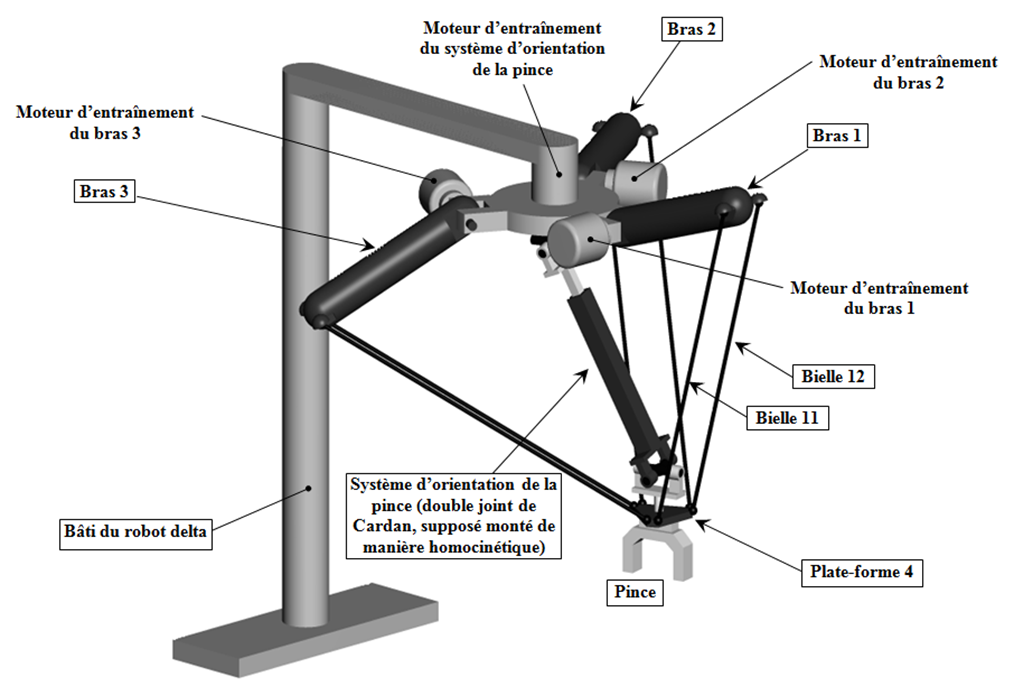
\includegraphics[width=.6\linewidth]{fig_01}
}%figues de la page de garde

\def\xxtitreexo{Radar d'avion}
\def\xxsourceexo{\hspace{.2cm} \footnotesize{F. Mathurin}}

\input{\repRel/Style/pagegarde_TD}

\setlength{\columnseprule}{.1pt}

\pagestyle{fancy}
\thispagestyle{plain}


\vspace{4.5cm}

\def\columnseprulecolor{\color{bleuxp}}
\setlength{\columnseprule}{0.4pt} 

%%%%%%%%%%%%%%
\setcounter{numques}{0}
\begin{multicols}{2}
Le support d'étude est un radar d'avion. Il permet au pilote de connaître la position des engins extérieurs (avions, hélicoptères, bateaux, ...). L'objectif de cette étude est de vérifier les performances décrites dans l’extrait de cahier des charges de ce système. 

\begin{center}
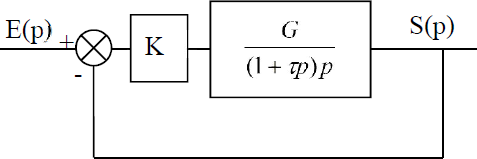
\includegraphics[width=\linewidth]{fig_02}
%\textit{}
\end{center}

On réalise un asservissement de position angulaire du radar d’avion : l'angle souhaité est $\theta_c (t)$, l'angle réel du radar est $\theta_r (t)$. La différence des deux angles est transformée en une tension $u_m (t)$, selon la loi $u_m (t)= A(\theta_c - \theta_r (t))$. La tension $u_m (t)$ engendre, via un moteur de fonction de transfert $H_m (t)$, une vitesse angulaire $\omega_m (t)$. Cette vitesse angulaire est réduite grâce à un réducteur de vitesse, selon la relation $\omega_r (t) = B \omega_m (t)$ ($B<1$), $\omega_r (t)$ étant la vitesse angulaire du radar. 

\question{Réaliser le schéma-bloc du système. }

Les équations du moteur à courant continu, qui est utilisé dans la motorisation, sont les suivantes : 
$$
u_m(t)=e(t)+Ri(t) 
\quad e(t)=k_e\omega_m(t) 
$$
$$J \dfrac{\text{d}\omega_m(t)}{\text{d}t} = c_m(t)
\quad c_m(t) = k_m i(t)
$$


Avec : 
\begin{itemize}
\item $u(t)$ : tension aux bornes du moteur (en V) (entrée du moteur);
\item $e(t)$ : force contre-électromotrice (en V);
\item $i(t)$ : intensité (en A);
\item $\omega_m (t)$ : vitesse de rotation du moteur (en rad/s);
\item $C_m (t)$ : couple moteur (en N.m) (un couple est une action mécanique qui tend à faire tourner); 
\item $J$ : inertie équivalente en rotation de l’arbre moteur (en $\text{kg.m}^2$): 
\item $R$ : résistance électrique du moteur;
\item $k_e$ : constante de force contre-électromotrice;
\item $k_m$ : constante de couple.
\end{itemize}


\question{Déterminer la fonction de transfert $H_m(p)=\dfrac{\Omega_m(p)}{U_m(p)}$.}

\question{Montrer que $H_m(p)$ peut se mettre sous la forme canonique $H_m(p)=\dfrac{K_m}{1+T_m p}$ et déterminer les valeurs littérales de $K_m$ et $T_m$.}



\question{En considérant la réponse indicielle d'un système, préciser la valeur de $\omega_m (t)$ à l'origine, la pente de la tangente à l'origine de $\omega_m (t)$ et la valeur finale atteinte par $\omega_m (t)$ quand t tend vers l’infini. }

\question{Déterminer la fonction de transfert $H(p)=\dfrac{\theta_r(p)}{\theta_c(p)}$. Montrer que cette fonction peut se mettre sous la forme d'un système du second ordre dont on précisera les caractéristiques.}

  La réponse indicielle de $H(p)$ à un échelon unitaire est donnée sur la figure suivante : 
  
\begin{center}
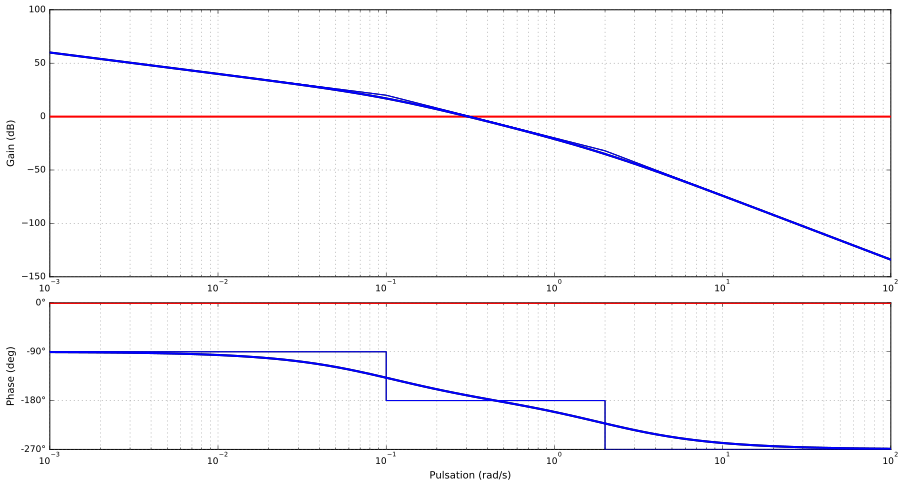
\includegraphics[width=\linewidth]{fig_03}
%\textit{}
\end{center}


\question{Déterminer, en expliquant la démarche utilisée, les valeurs numériques de $K$, $z$ et $\omega_0$.}

   Sans préjuger du résultat trouvé dans la question précédente, on prendra, pour la suite : $K = 1$, $z = 0,5$ et $\omega_0 = \SI{15}{rad/s}$.


\question{Déterminer, en expliquant la démarche utilisée, le temps de réponse à 5\%. Conclure quant la capacité du radar à vérifier le critère de rapidité du cahier des charges. }

On améliore la performance du radar en ajoutant un composant électronique (un correcteur) entre l'amplificateur et le moteur. La nouvelle fonction de transfert est : 
$
H(p)=\dfrac{1}{\left(1+0,05p \right)\left(1+0,0005p \right)\left(1+0,002p \right)}
$.
 

\question{Tracer le diagramme de Bode asymptotique (en gain et en phase) de cette fonction de transfert.}

\question{Déterminer $G$ et $\varphi$ pour $\omega = \SI{10}{rad/s}$.}
\question{Déterminer, en régime permanent, $\theta_r (t)$ pour une entrée $\theta_c (t) = 0,2 \sin(10t)$.}

Pour $\omega < \SI{20}{rad/s}$, on a $H(p)\simeq \dfrac{1}{1+0,05p}$.

\question{Déterminer, sur cette approximation, la pulsation de coupure à $-\SI{3}{dB}$. Conclure quant à la capacité du radar à satisfaire le critère de bande passante du cahier des charges.  }

\question{Déterminer, sur cette approximation, le temps de réponse à 5\% du système. Conclure quant à la capacité du radar à satisfaire le critère de rapidité du cahier des charges. }

\end{multicols}

\begin{center}
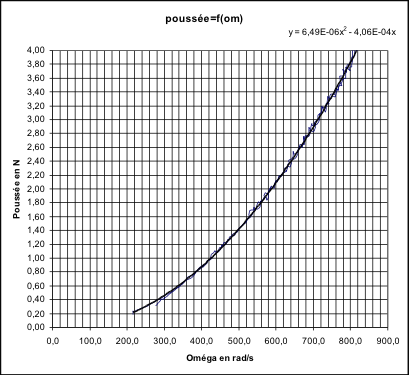
\includegraphics[width=\linewidth]{fig_04}
%\textit{}
\end{center}


%\end{document}
%
%\question{}
%
%
%\begin{center}
%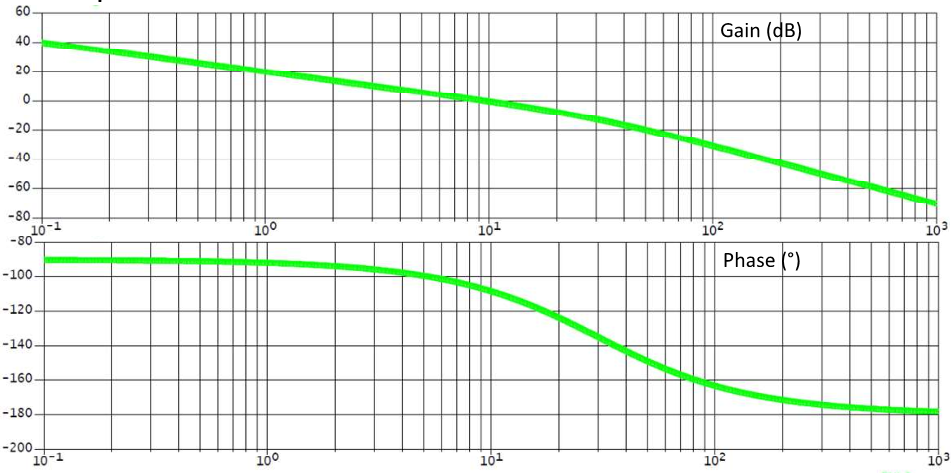
\includegraphics[width=\linewidth]{fig_06}
%%\textit{}
%\end{center}
%\begin{center}
%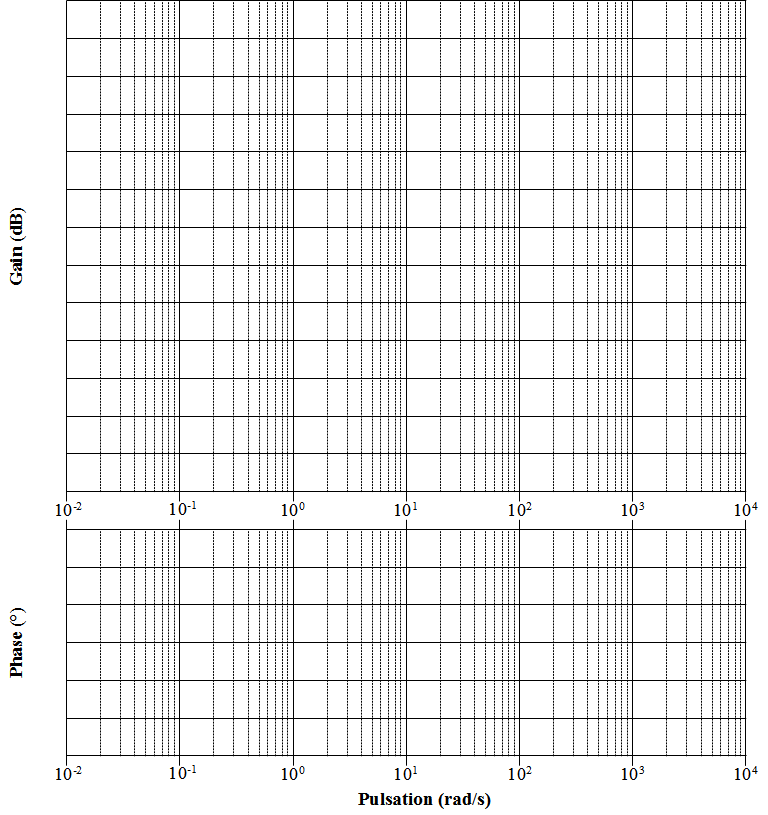
\includegraphics[width=\linewidth]{img_04}
%%\textit{}
%\end{center}

